The Birch--Swinnerton-Dyer conjecture is one the most important and celebrated statements in classical algebraic number theory, and has been driving large amounts of current research in the area. The statement conjecturally provides a bridge between the arithmetic of elliptic curves, or abelian varieties more generally, and the properties of their associated L-functions, a (conjecturally) meromorphic function in the complex plane, and therefore an analytic object in nature. This connection between arithmetic and analytic objects is ubiquitous throughout pure mathematics, and it has remarkable and surprising consequences, many of which are deep and non-trivial. The BSD conjecture for elliptic curves establishes the following connection.

\begin{conj}[BSD Conjecture]
    Let $E$ be an elliptic curve over a number field $F$, and let $L(E/F,s)$ be the associated L-function. Then
    \begin{equation}\label{eqn_BSD1}\tag{BSD1}
        \quad\ord_{s=1}L(E/F,s)=\rk E/F,
    \end{equation}
    and the leading term of the Taylor series at $s=1$ of $L(E/F,s)$ is given by
    \begin{equation}\label{eqn_BSD2}\tag{BSD2}
        \lim_{s\to1}\frac{L(E/F,s)}{(s-1)^r}\cdot\frac{\sqrt{|\Delta_F|}}{\Omega_+(E)^{r_1+r_2}|\Omega_-(E)|^{r_2}}=\frac{\Reg_{E/F}|\Sha_{E/F}|C_{E/F}}{|E(F)_{\tors}|^2},
    \end{equation}
    where $r$ is the order of the zero of $L(E/F,s)$ at $s=1$, $(r_1,r_2)$ is the signature of $F$, $\Omega_{\pm}$ are the periods of $E$, $\Reg_{E/F}$ is the regulator, $\Sha_{E/F}$ is the Tate-Shafarevich group and $C_{E/F}$ is a product of local terms depending on the primes in $F$ of bad reduction over $E$ (see Section \ref{sec_BSD}).
\end{conj}

In this document, we investigate the arithmetic consequences of the factorization of L-functions of elliptic curves over number fields, commonly known as Artin formalism. Dokchitser, Evans and Wiersema in \cite{DEW1} have already studied some of these and, in particular, they constructed a test that predicts positive rank for families of elliptic curves, which is only dependent on certain local arithmetic data associated to the primes of bad reduction of the elliptic curve. The existence of such tests, which we call `Norm Relations tests', is encoded in the following statement. 

\begin{conj}\cite[Theorem 33]{DEW1}\label{conj_normstest}
    Let $E/\QQ$ be an elliptic curve, $F/\QQ$ a finite Galois extension with Galois group $G$, $\rho$ an Artin representation over $\bQ$ that factors through $G$ and 
    \begin{equation}\label{eqn_localterms}\tag{\textdagger}
        \left(\bigoplus_{\mathfrak{g}\in\Gal(\QQ(\rho)/\QQ)}\rho^{\mathfrak{g}}\right)^{\oplus m}=\bigoplus_i\Ind_{F_i/\QQ}\mathds{1}\ominus\bigoplus_j\Ind_{F'_j/\QQ}\mathds{1}
    \end{equation}
    for some $m\geq 1$ and subfields $F_i,F'_j\subseteq F$. If either $\frac{\prod_i C_{E/F_i}}{\prod_j C_{E/F'_j}}$ is not a norm from some quadratic subfield $\QQ(\sqrt{D})\subseteq\QQ(\rho)$, or if it is not a rational square when $m$ is even, then $E$ has a point of infinite order over $F$.
\end{conj}

In the above conjecture, $\QQ(\rho)$ is the field obtained by attaching $\{\Tr(\rho(\fg)):\fg\in\Gal(K/\QQ)\}$, which is a Galois abelian extension of $\QQ$, and $\rho^{\fg}$ is the representation with character given by $\Tr\circ\rho^{\fg}=(\Tr\circ\rho)^{\fg}$ for $\fg\in\Gal(\QQ(\rho)/\QQ)$, denoted as the twist of $\rho$ by $\fg$.

%% This conjecture holds given stuff

Let us briefly describe an example where Conjecture \ref{conj_normstest} indeed predicts positive rank. We revisit this example in detail in Section \ref{sec_examples}.

\begin{example}[Example \ref{ex-C2C6}]
    Let $F/\QQ$ be a finite Galois extension such that $\Gal(F/\QQ)=C_2\times C_6$, which has the following subfield diagram.
    \begin{figure}[H]
        \centering
        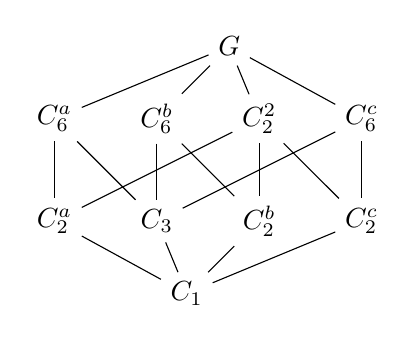
\begin{tikzpicture}[node distance=1.3cm]
            \node(G)[midway]{$G$};
            \node(C6b)[below left of =G]{$C_6^{b}$}; \node(C6a)[left of=C6b]{$C_6^{a}$};  
            \node(C22)[right of=C6b]{$C_2^{2}$};    \node(C6c)[right of=C22]{$C_6^{c}$};
            \node(C2a)[below of=C6a]{$C_2^{a}$};    \node(C3)[below of=C6b]{$C_3$};
            \node(C2b)[below of=C22]{$C_2^{b}$};    \node(C2c)[below of=C6c]{$C_2^{c}$};
            \node(C1)[below left of=C2b]{$C_1$};
            \draw(G)--(C6a);    \draw(G)--(C6b);    \draw(G)--(C6c);    \draw(G)--(C22);
            \draw(C6a)--(C2a);  \draw(C6a)--(C3);
            \draw(C6b)--(C2b);  \draw(C6b)--(C3);
            \draw(C6c)--(C2c);  \draw(C6c)--(C3);
            \draw(C22)--(C2a);  \draw(C22)--(C2b);  \draw(C22)--(C2c);
            \draw(C2a)--(C1);   \draw(C2b)--(C1);   \draw(C2c)--(C1);   \draw(C3)--(C1); 
        \end{tikzpicture}
    \end{figure}
    Let $E/\QQ$ be an elliptic curve such that it has multiplicative reduction at a prime $p$ with decomposition group $G$ and inertia group $C_6^b$ and such that every other prime of bad reduction is unramified in $F/\QQ$. If $\rho$ is an order $6$ character of $G$ with kernel $C_2^a$, then $\QQ(\rho)=\QQ(\zeta_6)=\QQ(\sqrt{-3})$. Following Conjecture \ref{conj_normstest}, we aim to compute 
    \begin{equation*}\label{eqn-rel2}
        \left(\frac{C_{E / F^{C_2^a}} C_{E / \bQ} }{C_{E / F^{C_6^a}} C_{E / F^{C_2^2}}}\right) \cdot \left( \frac{C_{E / F^{C_3}} C_{E / \bQ}^2}{C_{E / F^{C_6^a}}C_{E / F^{C_6^b}}  C_{E / F^{C_6^c}} } \right).
    \end{equation*}
    We remark that the underlying fields do satisfy the condition \eqref{eqn_localterms} from Conjecture \ref{conj_normstest}. This evaluates to $2\cdot\square$, and since $2$ is not a norm of an element from $\QQ(\sqrt{-3})$, Conjecture \ref{conj_normstest} forces $\rk E/F>0$. 
\end{example}

This test of predicting positive rank for families of elliptic curves should be reminiscent of using root number computations to predict positive rank based on local data. One takes the product of local roots numbers to obtain a global root number $w(E/K)\in{\pm1}$, and this arises in the (conjectural) functional equation of $L(E/K,s)$ (see Conjecture \ref{conj_hasseweil}). Hence, it describes the parity of the vanishing of the L-function at $s=1$. Assuming BSD, one expects the following to hold.

\begin{conj}[Parity Conjecture]\label{conj_parity}
    Let $E$ be an elliptic curve over a number field $K$. Then
    $(-1)^{\rk E / K} = w(E / K).$
\end{conj}

Using the Parity Conjecture to test for rank growth is known as a `parity test'. The Parity Conjecture has been extensively studied in the literature, see for example \cite{Tim} It is known to hold in certain conditions under the assumption of finiteness of $\Sha_{E/F}$. One can observe that the rank growth in the above example can also be explained by the Parity Conjecture, and we expect this phenomenon to happen in general. 

\begin{conj}\label{conj_normroot}
    Consider an elliptic curve $E / \bQ$, $F / \bQ$ a finite Galois extension, and relation 
    $$\left(\bigoplus_{\mathfrak{g}\in\Gal(\QQ(\rho)/\QQ)}\rho^{\mathfrak{g}}\right)^{\oplus m}=\bigoplus_i\Ind_{F_i/\QQ}\mathds{1}\ominus\bigoplus_j\Ind_{F'_j/\QQ}\mathds{1}$$
    as in \eqref{eqn_localterms}. If the product $\frac{\prod_i C_{E/F_i}}{\prod_j C_{E/F'_j}}$ is not a norm from some quadratic subfield $\QQ(\sqrt{D})\subseteq\QQ(\rho)$, or if it is not a rational square when $m$ is even, then there exists a subfield $K\subseteq F$ such that $w(E/K)w(E/\QQ)=-1$. 
\end{conj}

In Section \ref{sec-norm-rels-test} we describe a refined version of this conjecture, where it is phrased in terms of Artin twists of root numbers.

Parity tests cannot predict rank growth of elliptic curves in odd degree extensions. This is a direct consequence of the fact that odd degree groups have no non-trivial self dual representations (see Lemma \ref{lem_oddroot}). Accordingly, Norm Relations tests cannot make such a prediction either.

\begin{thm}[Theorem \ref{odd-exts}]\label{thm_odd-cons}
    Let $E / \bQ$ be an elliptic curve and let $F / \bQ$ be a Galois extension of odd order with Galois group $G$. Assume that $E$ has semistable reduction at $2$ and $3$ and take any representation $\rho$ of $G$. Suppose $m\geq 1$ and $F_i,F_j'\subseteq F$ satisfy 
    \begin{equation*}%\label{odd-exp} 
        \left(\bigoplus_{\mathfrak{g}\in\Gal(\QQ(\rho)/\QQ)}\rho^{\mathfrak{g}}\right)^{\oplus m }=\bigoplus_i\Ind_{F_i/\QQ}\mathds{1}\ominus\bigoplus_j\Ind_{F'_j/\QQ}\mathds{1}.
    \end{equation*}
    Then, for any $\QQ(\sqrt{D})\subseteq\QQ(\rho)$, we have that
    \[ \frac{\prod_i C_{E/F_i}}{\prod_j C_{E/F_j'}}  \in 
       \begin{cases}
           N_{\bQ(\sqrt{D}) / \bQ}(\bQ(\sqrt{D})^{\times}) & m \ \text{odd}, \\
           (\bQ^{\times})^2 & m \ \text{even}.
       \end{cases} 
    \] 
       %In other words, one cannot use Theorem \ref{thm_positive_rank} to conclude that $E / F$ must have positive rank. 
\end{thm}

%and this is indeed the case. In Sections \ref{sec_cyclic} and \ref{sec_odd} we describe two general settings in which Norm Relation test can never predict rank growth. One such setting is odd degree extensions.

The other setting in which Norm Relation tests cannot predict rank growth is when $F/\QQ$ is a Galois cyclic extension. When $G=\Gal(F/\QQ)$ is even and cyclic, parity tests can predict rank growth through the sign representation, which is a self-dual representation. However, for Norm Relation tests, the following holds.

\begin{thm}[Theorem \ref{thm_consistent_cyclic}]\label{thm_cyclic-cons}
    Let $d\geq2$ be a positive integer and let $F/K$ be a Galois extension of number fields such that $\Gal(F/K)=C_d$. Take any representation $\rho$ of $C_d$ and any semistable elliptic curve $E/\QQ$ at $2$ and $3$. 
    
    Let $F_i,F_j'$ be the intermediate fields of $F/K$ (which exist and are unique up to permutation) such that 
    \begin{equation*}%\label{odd-exp} 
        \bigoplus_{\mathfrak{g}\in\Gal(\QQ(\rho)/\QQ)}\rho^{\mathfrak{g}}=\bigoplus_i\Ind_{F_i/K}\mathds{1}\ominus\bigoplus_j\Ind_{F'_j/K}\mathds{1}
    \end{equation*}
    Then, for any $\QQ(\sqrt{D})\subseteq\QQ(\rho)$, we have that
    $$\frac{\prod_i C_{E/F_i}}{\prod_j C_{E/F_j'}}\in N_{\QQ(\sqrt{D})/\QQ}(\QQ(\sqrt{D})^{\times}).$$
\end{thm}

The strategy to prove these results is to break down the product 
$$\frac{\prod_i C_{E/F_i}}{\prod_j C_{E/F_j'}}=\prod_{\pp}\left(\frac{\prod_i \Cp(E/F_i)}{\prod_j \Cp(E/F_j')}\right)$$
into the local contributions of each prime $\pp$ in the base field (see Notation \ref{not_contr}). Each one of these local factors depends on the decomposition group $D_\pp\leq G$ and inertia group $I_\pp\triangleleft D_\pp$. Consequently, the following corollary also holds.

\begin{cor}[Corollary \ref{cor-odd-cyclic-decomp}]%\label{cor-odd-cyclic-decomp}
    Let $E / \bQ$ be an elliptic curve, $F / \bQ$ a Galois extension with Galois group $G$. Assume that $E$ has good or multiplicative reduction at $2$ and $3$. 
    
    Let $\rho$ be a representation of $G$, and let $m\geq 1$ and $F_i,F_j'\subseteq F$ be as in \eqref{eqn_localterms}. Let $p$ be a rational prime and suppose that $D_p\leq G$ is either cyclic or a group of odd order. Then, for any $\QQ(\sqrt{D})\subseteq\QQ(\rho)$, one has
    \[
        \frac{\prod_i C_{\fP\mid p}(E/F_i)}{\prod_j C_{\fP\mid p}(E/F_j')}\in
        \begin{cases}
            N_{\QQ(\sqrt{D})/\QQ}(\QQ(\sqrt{D})^{\times}) & \text{ $m$ odd,}\\ \QQss & \text{ $m$ even.}
        \end{cases}
    \] 
\end{cor}

Therefore, when trying to use Norm Relations tests to force positive rank, interesting cases can only occur when $E/\QQ$ has bad reduction at primes that ramify in $F/\QQ$ and such that $D_p$ is non-cyclic and has even order.

\subsection*{Layout of the Report}
The purpose of this project is two-fold: firstly, it aims to serve as an introduction to the topics related to the Birch--Swinnerton-Dyer conjecture and, secondly, it studies the arithmetic consequences of Conjecture \ref{conj_normstest} for elliptic curves.

Sections \ref{sec_EC} to \ref{sec_BSD} serve the first purpose. In Section \ref{sec_EC}, we give a brief and rather informal discussion on the theory of elliptic curves, where we dedicate most of our attention in describing their local behaviour. 
%Of course, we assume familiarity with the topic, but we give appropriate references for those results that are generally less known or harder to find in the literature. 
In Section \ref{sec_Lside}, we introduce the notion of an Artin representation and $\ell$-adic representation, and we also give a detailed description on the construction of the L-functions $L(E/F,s)$ associated to an elliptic curve over a number field $F$ and of its twist by an Artin representation $\rho$. Finally, in Section \ref{sec_BSD} we discuss the BSD conjecture in more detail and we explain the arithmetic terms appearing in the statement of the conjecture. We also discuss an important conjectural analogue of BSD for Artin twists which naturally leads to the statement of Conjecture \ref{conj_4}, which motivates the latter half of the discussion.

The remaining sections serve the second purpose of studying the arithmetic of elliptic curves through Conjecture \ref{conj_4}. In Section \ref{sec_pos_rank} we describe how to derive Conjecture \ref{conj_normstest} from the statement of Conjecture \ref{conj_4}, and we provide detailed examples on how Norm Relations test predict positive rank. The statement and proofs of Theorems \ref{thm_odd-cons} and \ref{thm_cyclic-cons} are more naturally phrased in representation theoretic terms. Therefore, in Section \ref{sec_norm}, we introduce the necessary notation and results required for the later sections. 

The last three sections of the report are devoted to proving Theorems \ref{thm_odd-cons} and \ref{thm_cyclic-cons}. In Section \ref{sec_preliminary}, we prove some preliminary results that describe the local behaviour of some families of elliptic curves. Sections \ref{sec_cyclic} and \ref{sec_odd} contain the main proofs of the report on the cyclic and odd cases, respectively. At the end of the report, the reader can find the Appendix with some global class field theory that are used throughout the latter sections.

\subsection*{Acknowledgements}

We would like to thank our supervisor Vladimir Dokchitser for his generosity with his time, his many helpful suggestions, and for introducing us to this interesting topic.
